
\section{Fortbewegung}

\subsection{Fahrrad}

Fahrradfahren lohnt sich nicht nur, weil es die schnellste und
flexibelste M�glichkeit ist, in M�nchen voranzukommen, es ist auch
gesund, schont das Klima und macht Spa�.  Es ist auch deutlich
g�nstiger als die h�ufig �berf�llten �ffentlichen Nahverkehrsmittel:
Drei Monate Fahrrad statt MVG und schon hast du mindestens 100~�
gespart.

Damit kann man schon den ein oder anderen Drahtesel refinanzieren oder
hat zumindest eine Anzahlung f�r ein gutes, gebrauchtes Fahrrad. Diese
findet man beispielsweise bei eBay, Polizei-, Bahnhofs- und
Wohnheimversteigerungen oder auf einem der zahlreichen Flohm�rkte in
M�nchen. Kleiner Tipp: Beschr�nke dich bei der Suche nicht nur auf die
Stadt, sondern beziehe das Umland mit ein. Dort findet man oft
deutlich bessere Angebote.

\paragraph{Hier noch ein paar Tipps f�r den M�nchner Stra�enverkehr:}
\begin{itemize}
	\item Um Trambahnschienen sollte man nicht nur bei Regen und Gl�tte einen gro�en Bogen machen.
	\item Fu�g�nger sind in ihrem Verhalten unvorhersehbar. Die Autofahrer leider auch.
	\item Mit Licht und Helm fahren kann dein Leben retten.
	\item Um das Wiederfinden des Fahrrades zu erleichtern, sollte man es abschlie�en.
	\item M�nchen ist nicht nur Radlhauptstadt, sondern auch (gef�hlte) Kontrollierhauptstadt:

	\begin{itemize}
        	\item Auf der richtigen Stra�enseite fahren -- insbesondere auf der Leopold- / Ludwigstr. (15~�).
	        \item Nicht bei Rot �ber die Ampel fahren (min. 90~� und ein paar Punkte in Flensburg).
	        \item In der Innenstadt Schrittgeschwindigkeit einhalten, wo es ausgeschildert ist (15~�).
	        \item Nicht ohne Licht durch Nacht und Dunkelheit (15~�).
	\end{itemize}
\end{itemize}

%\begin{textblock*}{\paperwidth}(50mm,128mm)
%   \noindent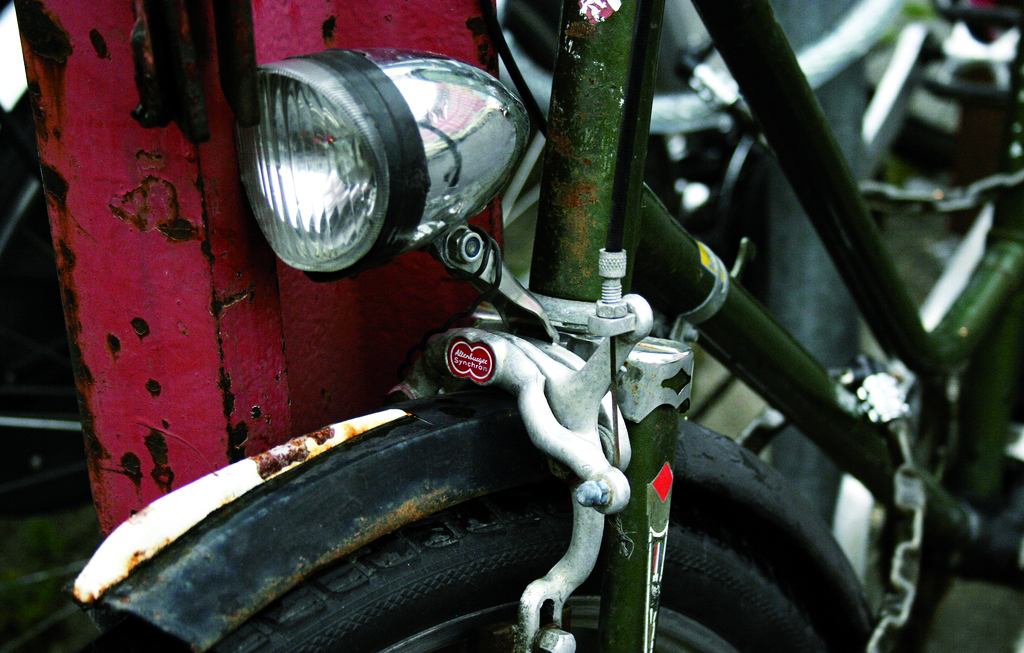
\includegraphics[width={\paperwidth-50mm}]{flickr/725703538_5b9a97ecf2_b}
%	\label{img_bike}
%\end{textblock*}

\clearpage

\subsection{MVV}

\paragraph{Mit den �ffentlichen Verkehrsmitteln in die Uni}\hfill\\
Mit der U3 bzw. U6 Haltestelle Universit�t kommst du direkt zum Hauptgeb�ude. Zu den meisten anderen Geb�uden kommst du von dort aus relativ schnell. F�r diese gibt es aber meistens auch n�herliegende Haltestellen, welche man auch auf der Karte in diesem Heft finden kann.

\paragraph{Kosten}\hfill\\
F�r die meisten Studenten ist momentan der von der MVV (M�nchner Verkehrsverbund) angebotene Ausbildungstarif II am interessantesten. Der Preis richtet sich dabei nach der Zahl der ben�tigten Zeitkartenringe, die befahren werden. Bevor du dir aber ein Ticket kaufen kannst, musst du dir ein Kundenkarte besorgen. Diese bekommst du im MVG-Kundencenter am Hauptbahnhof, Ostbahnhof oder in der Poccistr.~1--3 (alle zwischen 8:00 und 18:00~Uhr) oder online \newline http://www.mvv-muenchen.de/de/tickets-preise/tickets/schule-ausbildung-und-studium/\newline kundenkarte/index.html\#c9815

Das Ticket gibt es mit der G�ltigkeit einer Woche (9,50 -- 38,90~�) oder eines Monats (34,70 -- 142,00~�) an einem der MVG-Zeitkartenautomaten, in den MVG-Kundencentern oder den MVG-Verkaufsstellen. Monatsfahrkarten gelten bis 12Uhr des ersten Werktags des Folgemonats.\\
~
Wenn du in Zukunft g�nstiger unterwegs sein willst, kannst du bei der Initiative Ausbildungsticket, einem B�ndnis aus Studenten, Sch�lern und Azubis mitmachen:\newline \url{ausbildungsticket.de}

Mehr Infos zum Ausbildungstarif: \url{mvg-mobil.de/tarife/ausbildungstarif.html}


\subsection{Auto}
Du kommst im Allgemeinen mit dem Auto nicht schneller durch die Stadt, als mit dem �PNV oder dem Fahrrad. Sp�testens bei der Parkplatzsuche vor der Uni wirst du dann merken, dass es bessere M�glichkeiten gibt, an die Uni zu kommen.
